\documentclass[tikz,crop,convert={density=200,outext=.png},border=0.4cm]{standalone}

\usepackage{pgfplots}
\usepackage{amsmath}
\usetikzlibrary{arrows.meta}
\usepackage{physics}
\usepackage{xcolor}
\definecolor{pow_1}{RGB}{103,0,31}
\definecolor{pow_2}{RGB}{206,18,86}
\definecolor{pow_3}{RGB}{223,101,176}
%\definecolor{pow_1}{RGB}{73,0,106}
%\definecolor{pow_2}{RGB}{174,1,126}
% \definecolor{pow_3}{RGB}{221,52,151}
%\definecolor{pow_3}{RGB}{247,104,161}
\pgfplotsset{compat=newest,
    %width=6cm,
    %height=3cm,
    scale only axis=true,
    max space between ticks=25pt,
    try min ticks=5,
    every axis/.style={
        axis y line=middle,
        axis x line=middle,
        axis line style={thick,->,>=latex, shorten >=-.3cm}
    },
    every axis plot/.append style={thick},
    tick style={black, thick},
}
\tikzset{
    semithick/.style={line width=0.8pt},
}
\usepgfplotslibrary{groupplots}
\usepgfplotslibrary{dateplot}
% Document begins
\begin{document}
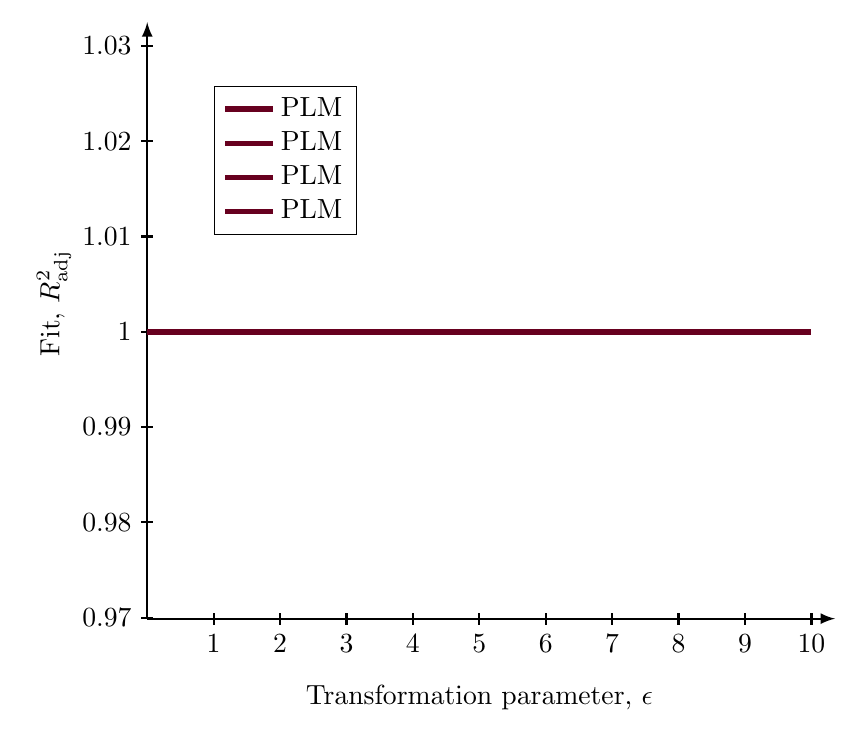
\begin{tikzpicture}
  % The axis of the plot
\begin{axis}[
    %title={Model: $\dv{y}{t}=\frac{2y}{t}$ with solution $y(t)=C_1t^2$\\Symmetry: $\Gamma_{\epsilon}=(t,y)\mapsto\left(\exp\left(\epsilon\right)t,\exp\left(-\epsilon\right)y\right)$},
    title style = {align=left},
    xlabel={Transformation parameter, $\epsilon$},
    % ylabel={Sum of the squared residuals, $SS(\epsilon)$},
    % ylabel={The root mean square RMS, $\rho_0$},
    ylabel={Fit, $R^{2}_{\mathrm{adj}}$},
    %ylabel={Logarithm of Incidence, $\ln\left(R(t)\right)$},        
    x label style={at={(axis description cs:0.5,-0.1)},anchor=north},
    y label style={at={(axis description cs:-0.1,0.55)},rotate=90,anchor=south},    
    %xmin=0, xmax=125.5,
    % xmin=-27, xmax=5,
    % ymin=0, ymax=560,
    ymin=0.9699, ymax=1.03,
    %xtick={-30,-27,...,9},
    %xtick={0,12,20,...,60,70,82},    
    %ytick={-15,-10,...,15},
    %legend style={at={(axis description cs:0.05,0.9)},anchor=west},    
    %legend style={at={(axis description cs:0,0.8)},anchor=west},
    legend style={at={(axis description cs:0.1,0.8)},anchor=west},    
    %legend pos=north west,
    %ymajorgrids=true,
    grid style=dashed,
]
% Plot the model
\addplot[
color=pow_1,line width=2pt,
]
coordinates {%
(0.0,1.0)
(0.5263157894736842,1.0)
(1.0526315789473684,1.0)
(1.5789473684210527,1.0)
(2.1052631578947367,1.0)
(2.631578947368421,1.0)
(3.1578947368421053,1.0)
(3.6842105263157894,1.0)
(4.2105263157894735,1.0)
(4.7368421052631575,1.0)
(5.263157894736842,1.0)
(5.789473684210526,1.0)
(6.315789473684211,1.0)
(6.842105263157895,1.0)
(7.368421052631579,1.0)
(7.894736842105263,1.0)
(8.421052631578947,1.0)
(8.947368421052632,1.0)
(9.473684210526315,1.0)
(10.0,1.0)
};
\addlegendentry{PLM}
\addplot[
color=pow_1,line width=2pt,
]
coordinates {%
(0.0,1.0)
(0.5263157894736842,1.0)
(1.0526315789473684,1.0)
(1.5789473684210527,1.0)
(2.1052631578947367,1.0)
(2.631578947368421,1.0)
(3.1578947368421053,1.0)
(3.6842105263157894,1.0)
(4.2105263157894735,1.0)
(4.7368421052631575,1.0)
(5.263157894736842,1.0)
(5.789473684210526,1.0)
(6.315789473684211,1.0)
(6.842105263157895,1.0)
(7.368421052631579,1.0)
(7.894736842105263,1.0)
(8.421052631578947,1.0)
(8.947368421052632,1.0)
(9.473684210526315,1.0)
(10.0,1.0)
};
\addlegendentry{PLM}
\addplot[
color=pow_1,line width=2pt,
]
coordinates {%
(0.0,1.0)
(0.5263157894736842,1.0)
(1.0526315789473684,1.0)
(1.5789473684210527,1.0)
(2.1052631578947367,1.0)
(2.631578947368421,1.0)
(3.1578947368421053,1.0)
(3.6842105263157894,1.0)
(4.2105263157894735,1.0)
(4.7368421052631575,1.0)
(5.263157894736842,1.0)
(5.789473684210526,1.0)
(6.315789473684211,1.0)
(6.842105263157895,1.0)
(7.368421052631579,1.0)
(7.894736842105263,1.0)
(8.421052631578947,1.0)
(8.947368421052632,1.0)
(9.473684210526315,1.0)
(10.0,1.0)
};
\addlegendentry{PLM}
\addplot[
color=pow_1,line width=2pt,
]
coordinates {%
(0.0,1.0)
(0.5263157894736842,1.0)
(1.0526315789473684,1.0)
(1.5789473684210527,1.0)
(2.1052631578947367,1.0)
(2.631578947368421,1.0)
(3.1578947368421053,1.0)
(3.6842105263157894,1.0)
(4.2105263157894735,1.0)
(4.7368421052631575,1.0)
(5.263157894736842,1.0)
(5.789473684210526,1.0)
(6.315789473684211,1.0)
(6.842105263157895,1.0)
(7.368421052631579,1.0)
(7.894736842105263,1.0)
(8.421052631578947,1.0)
(8.947368421052632,1.0)
(9.473684210526315,1.0)
(10.0,1.0)
};
\addlegendentry{PLM}

\end{axis}
\end{tikzpicture}

\end{document}
